\subsection{Rayleigh-Taylor Instability}

This problem consists on the evolution of two layers of fluids initially at rest in the gravity field. The top layer is more dense than the one is placed at the bottom. Due to a little disturbance in the contact surface the more dense fluid goes down and the less dense fluid does the opposite. In the intermediate state a mixture is created, which is lately segregated. The final state reaches an stable equilibrium with the more dense fluid at the bottom layer and the less dense fluid at the top layer. The growth and evolution of the instability has been investigated among others by Tryggvason\cite{Tryggvason88} for inviscid incompressible flows, and by Guermond
\& Quartapelle\cite{Guermond00} for viscous flows.

The starting point is the problem documented by Guermond. The domain is $[−d/2,-2d]\times[d/2,2d]$. The initial position of the perturbed interface is $\eta(x) = −0.1d \cos(2\pi x/d)$. The heavy fluid is above and the density ratio is $3$, so that the Atwood
number is $0.5$ according to Tryggvason's definition $At = (\rho_{max}-\rho_{min})/(\rho_{max}+\rho_{min})$. Other physical parameters are selected to obtain $Re=\rho_{min}d^{\frac{3}{2}}g^{\frac{1}{2}}/\mu=1000$. Computational domain is discretized into $160000$ structured triangles ($\Delta x=0.01$) setting slip boundary conditions on each wall. Time step selected is $\Delta t=0.01[s]$, which allows to reach $CFL_{max} \approx 8$.

To compare with reference results, the time is made dimensionless by using $\widetilde{t} = t\sqrt{g\ At}$. Results on the vertical position of the tip of the falling and rising fluid (spike and bubble, respectively) are shown in Figure \ref{fg:rayleigh-rf}. It can be observed that current solution is in good agreement with the reference results.

\begin{figure}[H]
  \begin{center}
      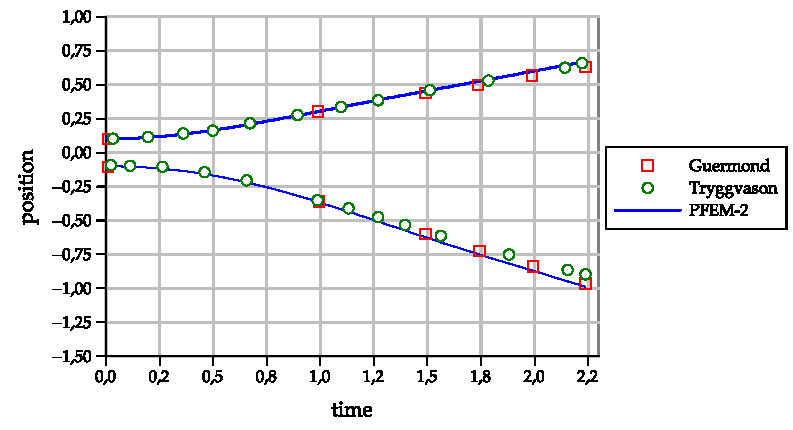
\includegraphics[width=\columnwidth]{images/rayleigh_1.pdf}
  \end{center}
  \caption{\label{fg:rayleigh-rf} Position of rising and falling bubbles versus time. Case with $Re=1000$.}
\end{figure}

On the other hand, the evolution of the instability is shown in Figure \ref{fg:rayleigh-screenshots} at dimensionless times $\widetilde{t}=0, 1, 1.5, 2$. Around $\widetilde{t}=1.5$ the heavy fluid begins to roll up into two counter-rotating vortices. Later, around $\widetilde{t} = 2$, these two vortices become unstable and a pair of secondary vortices appear at the tails of the roll-ups. These shapes of the fluid interface obtained with PFEM-2 are similar than those of the reference results.


\begin{figure}[htbp]
  \begin{center}
      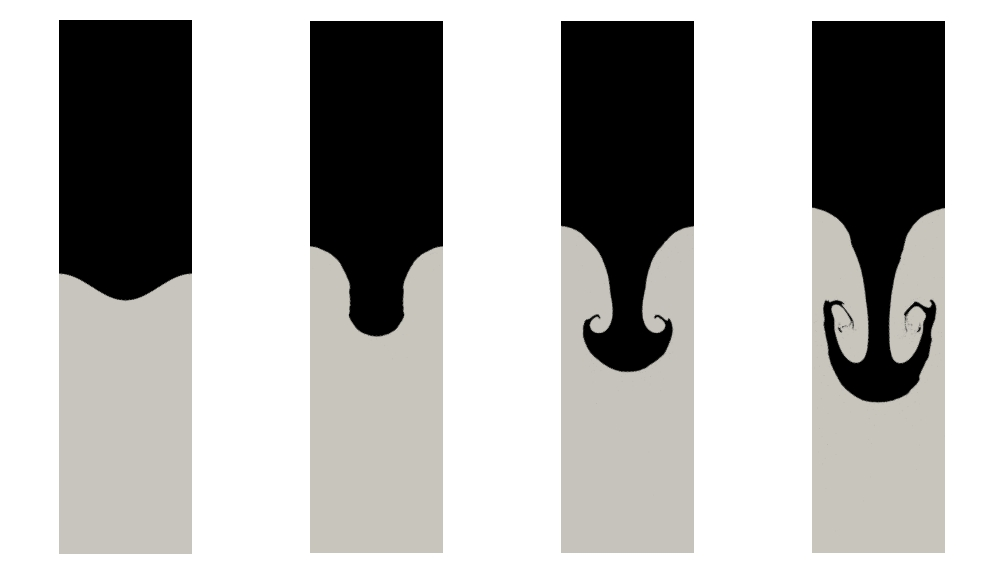
\includegraphics[width=\columnwidth]{images/rayleigh_2.jpg}
  \end{center}
  \caption{\label{fg:rayleigh-screenshots} Rayleigh-Taylor instability evolution. Case with $Re=1000$. From left to right $\widetilde{t} =0.0$, $1.0$, $1.5$, $2.0$.}
\end{figure}
\afterpage{\clearpage}

